\documentclass[11 pt]{article}
\usepackage{graphicx}
\title{
	My crypto libraries \\
	\large HW4 - CNS Sapienza}

\author{Giulia Muscarà 1743261}
\date{November 28, 2019}

\begin{document}

\maketitle

\section{Introduction}
The purpose of this report is to analyse two  Python and two C freely available cryptographic libraries, in particular with respect to their licenses, supported functions and API use for symmetric encryption/decryption, comparing them and making examples of use. These programming languages' libraries were chosen as they provide robust, efficient cryptographic algorithms and protocols.
 
\section{C cryptographic libraries}
The two chosen libraries for C were OpenSSL and WolfSSL.

\subsection{OpenSSL} 
OpenSSL is a software library providing functions to secure communications over computer networks against eavesdropping or to guarantee authentication. OpenSSL contains an open-source implementation of the SSL and TLS protocols. The C library  implements basic cryptographic functions and provides various utility functions and it is available for most Unix-like operating systems and Microsoft Windows. OpenSSL library has the following characteristics:
\begin{enumerate}
	\item Ciphers: AES, Blowfish, Camellia, Chacha20, Poly1305, SEED, ARIA, DES, IDEA, RC2, RC4, RC5, Triple DES, GOST 28147-89, SM4;
	\item Modes: ECB, CBC, CTR, OOFB, CFB, CCM, GCM, OCB, XTS;
	\item Cryptographic hash functions: MD5, MD4, MD2, SHA-1, SHA-2, SHA-3, RIPEMD-160, MDC-2, GOST R 34.11-94, BLAKE2, Whirlpool, SM3;
	\item Public-key cryptography: RSA, DSA, Diffie–Hellman key exchange, Elliptic curve, X25519, Ed25519, X448, Ed448, GOST R 34.10-2001, SM2;
	\item License: OpenSSL is double licensed under the OpenSSL License (Apache License 1.0) and the SSLeay License but next version will be relicensed under the terms of the Apache License 2.0.
\end{enumerate}

\subsection{WolfSSL} 
WolfSSL is a portable, embedded SSL/TLS library.  Written in C language, it includes SSL/TLS client libraries and a server implementation as well as support for multiple APIs. WolfSSL relies on WolfCrypt and NTRU cryptographic libraries and it supports a number of different cryptographic utilities:
\begin{enumerate}
	\item Ciphers: AES, RC4, DES and 3DES, Camellia and ChaCha20;
	\item Modes:ECB, CBC, CTR, CCM, GCM;
	\item Cryptographic hash functions: MD5, Blake2,	SHA1, SHA2, SHA-256, SHA-384, and SHA-512;
	\item Public-key cryptography: RSA, ECC,	ECC-DHE, Curve25519 and	Ed25519;
	\item License: GNU General Public License GPLv2. 
\end{enumerate}
Nettle also provide the PBKDF2 key derivation function and the POLY1305 and UMAC message authentication codes.\\

\subsection{OpenSSL vs WolfSSL}
OpenSSL and Nettle are both open source libraries. While Nettle is an attempt to avoid the problem of the overfitting of cyptographic libraries for particular applications by using  low-level cryptography and providing a simple and general interface to it, OpenSSL originally aimed to provide a free set of encryption tools for the code used on the Internet.
However, WolfSSL includes an OpenSSL compatibility interface with the most commonly used OpenSSL functions, so they are compatible and it was possible to switch from one library to the other to encrypt and decrypt in C, as it was done in the attached C code. The output of the execution is showed in Fig. 1.

\begin{figure}[!h]
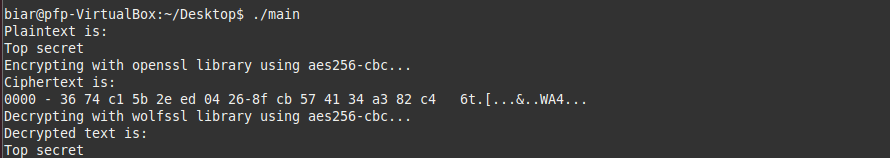
\includegraphics[width=1\textwidth]{c_output-hw4-1743261.png}
\caption{Switching of C crypto libraries}
\end{figure}

When compiling, the used libraries were linked as well, as shown in Fig. 2.\\


\begin{figure}[!h]
	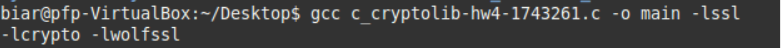
\includegraphics[width=1\textwidth]{c_link-hw4-1743261.png}
	\caption{Linking of C crypto libraries}
\end{figure}

\section{Python cryptographic libraries}
The two chosen libraries for Python were Cryptography and Pycrypto.

\subsection{Cryptography 2.8}
Cryptography is a package which provides cryptographic primitives for Python environment. It supports Python 2.7, Python 3.4+, and PyPy 5.4+. The 2.8 version of the library waas adopted. It includes both low and high level primitives and interfaces to common cryptographic algorithms. Cryptography library has the following characteristics:
\begin{enumerate}
	\item Ciphers: AES, TripleDES, Camellia, ChaCha20, CAST5, SEED, Bowfish, R4 and IDEA;
	\item Modes: CBC, CTR, OFB, CFB, CFB8, GCM;
	\item Cryptographic hash functions: SHA-2 and SHA-3 families, SHA1, BLAKE2 and MD5;
	\item Public-key cryptography: RSA, Diffie-Hellman key exchange, DSA, X25519 key exchange and X448 key exchange;
	\item License: from 2017, it has been relicensed under either the Apache Software License 2.0 or the BSD license.
\end{enumerate}

\subsection{Pycrypto}
The PyCrypto toolkit's purpose is to provide a reliable and stable base to use cryptographic functions in Python programs. It offers a simple and consistent interface for similar classes of algorithms. The currently available ciphers and features are listed below:
\begin{enumerate}
	\item Ciphers: AES, RC2, RC4, RC5, DES and TripleDES, XOR, Cast, Blowfish and IDEA;
	\item Modes: CBC, CTR, OFB, CFB, CFB8, GCM;
	\item Cryptographic hash functions: RIPEMD, SHA-1, SHA-256, MD2, MD4 and MD5;
	\item Public-key cryptography: RSA, ElGamal, qNEW and DSA;
	\item License: public domain.
\end{enumerate}

\subsection{Cryptography vs Pycrypto}
Cryptography and PyCrypto both share the goal of making an easier and safer cryptography library. However, cryptography is designed to be a general purpose library, interoperable with existing systems, while PyCrypto provides a smaller but still robust set of features.
Also in this case it was possible to encrypt using the former and then decrypting using the latter without any problem of incompatibility.\\
The resulting output is provided in Fig.3.\\\\\\\\\\\\

\begin{figure}[!t]
	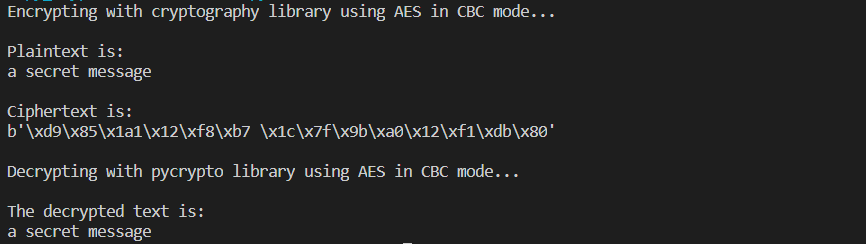
\includegraphics[width=1\textwidth]{py_output-hw4-1743261.png}
	\caption{Switching of Python crypto libraries}
\end{figure}

\begin{thebibliography}{10}

	\subsubsection*{Manuals and Docs}
	\bibitem{OpenSSL Manual}
	\textsl{OpenSSL} \\
	\textit{https://www.openssl.org/docs}
	
	\bibitem{WolfSSL Manual}
	\textsl{WolfSSL} \\
	\textit{https://www.wolfssl.com/docs/}
	
	\bibitem{Pycrypto Manual}
	\textsl{Pycrypto} \\
	\textit{https://www.dlitz.net/software/pycrypto/api/2.3/}
	
	\bibitem{Cryptography Manual}
	\textsl{Cryptography} \\
	\textit{https://cryptography.io/en/latest/}
	
\end{thebibliography}

\end{document}